% Standalone RAKL four-arm causal-attribution DESIGN (Paper III, Figure 5).
% Pre-registered structure, not yet executed: all result cells are empty by design.
% Build:  pdflatex four_arm_design.tex  -> four_arm_design.pdf
\documentclass[border=6pt]{standalone}
\usepackage{tikz}
\usepackage{helvet}\renewcommand{\familydefault}{\sfdefault}
\usetikzlibrary{positioning,arrows.meta,shapes.geometric,fit,backgrounds,calc}
\definecolor{oiblue}{HTML}{0072B2}
\definecolor{oivermillion}{HTML}{D55E00}
\begin{document}
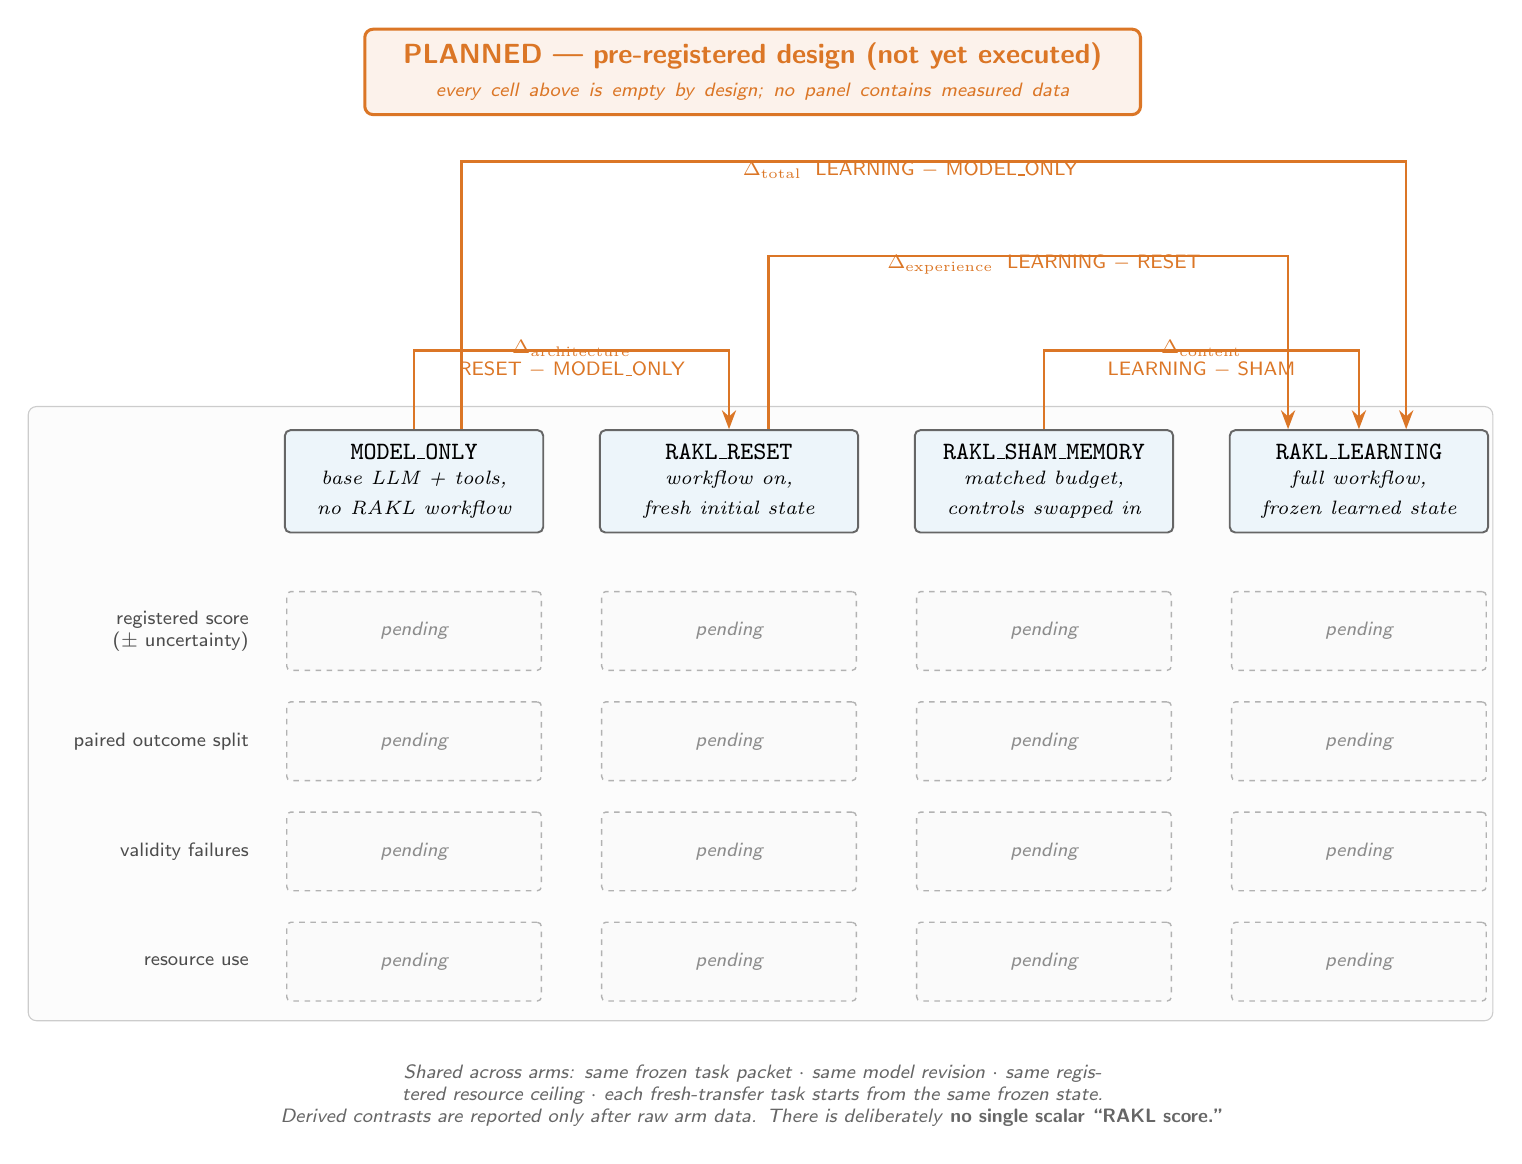
\begin{tikzpicture}[
  font=\small,
  >={Stealth[length=2.4mm]},
  head/.style={rounded corners=2pt, draw=black!60, line width=0.7pt, align=center,
               inner sep=4pt, minimum height=13mm, text width=30mm, fill=oiblue!7,
               font=\ttfamily\small},
  cell/.style={rounded corners=1.5pt, draw=black!30, dash pattern=on 2pt off 2pt,
               line width=0.5pt, align=center, minimum height=10mm, text width=30mm,
               fill=black!2, font=\scriptsize\itshape, text=black!45},
  rowlbl/.style={align=right, text width=26mm, font=\scriptsize, text=black!70},
  lift/.style={->, line width=0.9pt, draw=oivermillion!85},
  liftlbl/.style={font=\scriptsize, text=oivermillion!85, align=center},
  note/.style={font=\scriptsize\itshape, text=black!60},
]
% ---- geometry ----
\def\cA{0}   \def\cB{4}   \def\cC{8}   \def\cD{12}
\def\rH{0}   \def\rone{-1.9} \def\rtwo{-3.3} \def\rthree{-4.7} \def\rfour{-6.1}

% ---- column headers (the four arms) ----
\node[head] (h1) at (\cA,\rH) {MODEL\_ONLY\\[1pt]{\rmfamily\itshape\scriptsize base LLM + tools,\\no RAKL workflow}};
\node[head] (h2) at (\cB,\rH) {RAKL\_RESET\\[1pt]{\rmfamily\itshape\scriptsize workflow on,\\fresh initial state}};
\node[head] (h3) at (\cC,\rH) {RAKL\_SHAM\_MEMORY\\[1pt]{\rmfamily\itshape\scriptsize matched budget,\\controls swapped in}};
\node[head] (h4) at (\cD,\rH) {RAKL\_LEARNING\\[1pt]{\rmfamily\itshape\scriptsize full workflow,\\frozen learned state}};

% ---- row labels ----
\node[rowlbl] at (-3.4,\rone)  {registered score\\($\pm$ uncertainty)};
\node[rowlbl] at (-3.4,\rtwo)  {paired outcome split};
\node[rowlbl] at (-3.4,\rthree){validity failures};
\node[rowlbl] at (-3.4,\rfour) {resource use};

% ---- empty (pre-data) result cells : 4 arms x 4 metrics ----
\foreach \x in {\cA,\cB,\cC,\cD}{
  \node[cell] at (\x,\rone)  {pending};
  \node[cell] at (\x,\rtwo)  {pending};
  \node[cell] at (\x,\rthree){pending};
  \node[cell] at (\x,\rfour) {pending};
}

% ---- derived lift contrasts (arrows over the headers, stacked to avoid overlap) ----
% level 1 (up 1.0): architecture (1->2) and content (3->4) -- disjoint spans
\draw[lift] (h1.north) -- ++(0,1.0) -| (h2.north);
\node[liftlbl] at (\cB-2,1.55) {$\Delta_{\mathrm{architecture}}$\\{\scriptsize RESET $-$ MODEL\_ONLY}};
\draw[lift] (h3.north) -- ++(0,1.0) -| (h4.north);
\node[liftlbl] at (\cD-2,1.55) {$\Delta_{\mathrm{content}}$\\{\scriptsize LEARNING $-$ SHAM}};
% level 2 (up 2.2): experience (2->4)
\draw[lift] ($(h2.north)+(0.5,0)$) -- ++(0,2.2) -| ($(h4.north)+(-0.9,0)$);
\node[liftlbl] at (8,2.75) {$\Delta_{\mathrm{experience}}$\ \ {\scriptsize LEARNING $-$ RESET}};
% level 3 (up 3.4): total (1->4)
\draw[lift] ($(h1.north)+(0.6,0)$) -- ++(0,3.4) -| ($(h4.north)+(0.6,0)$);
\node[liftlbl] at (6.3,3.95) {$\Delta_{\mathrm{total}}$\ \ {\scriptsize LEARNING $-$ MODEL\_ONLY}};

% ---- grid background box ----
\begin{scope}[on background layer]
  \fill[black!1, rounded corners=3pt] (-4.9,0.95) rectangle (13.7,-6.85);
  \draw[black!20, rounded corners=3pt] (-4.9,0.95) rectangle (13.7,-6.85);
\end{scope}

% ---- PLANNED banner (top) ----
\node[draw=oivermillion!85, line width=1.1pt, rounded corners=3pt, fill=oivermillion!8,
      align=center, inner sep=5pt, font=\bfseries, text=oivermillion!85, text width=95mm]
      (banner) at (4.3,5.2)
      {PLANNED --- pre-registered design (not yet executed)\\
       {\normalfont\scriptsize\itshape every cell above is empty by design; no panel contains measured data}};

% ---- footer conditions / rules ----
\node[note, align=center, text width=150mm] at (4.3,-7.8)
      {Shared across arms: same frozen task packet\ $\cdot$\ same model revision\ $\cdot$\ same registered resource ceiling\ $\cdot$\
       each fresh-transfer task starts from the same frozen state.\\
       Derived contrasts are reported only after raw arm data. There is deliberately \textbf{no single scalar ``RAKL score.''}};
\end{tikzpicture}
\end{document}
